
\chapter{Application and Results} \label{chap:4}


\section{Marlim (or Pipesim) Simulator}
Sistemas de produção de petróleo são sistemas nos quais se deseja sempre produzir o máximo possível e de forma segura.
O PIPESIM, da Schlumberger, é um simulador de fluxo multifásico em regime permanente que pode ser utilizado tanto para o projeto como para planejamento de operações em campos de petróleo. Ele permite que sejam simuladas situações alternativas de forma mais rápida e segura que testes reais.



\section{Experimentos}
Foram realizados XX experimentos, em crescente ordem de complexidade

\subsection{Sintonia de curva }
Primeiramente foi configurado um unico poço de petróleo, que pode ser visto na figura \ref{fig:setup1_dia}. A seguir foram escolhidos dados arbitrariamente para compor a curva "real" de produção.
Neste Experimento a curva sintonizada foi a de fluxo de líquido (Barris padrões por dia) por gás injetado (milhões de pés cúbicos padrões por dia). Escolheu-se a pressão estática do reservatório como sendo 4000 psi absoluto, e um indice de produtividade liquido de 25 STDB/d/psi( Barris padrões por dia por pressão estática). Desta forma a figura \ref{fig:truth1} demonstra a curva "real" a ser sintonizada.

\begin{figure}
\centering
\begin{subfigure}{.4\textwidth}
  \centering
  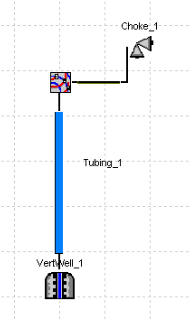
\includegraphics[height=1\linewidth]{figs/setup1.png}
  \caption{Setup do poço de petróleo.}
  \label{fig:setup1_dia}
\end{subfigure}%
\begin{subfigure}{.6\textwidth}
  \centering
  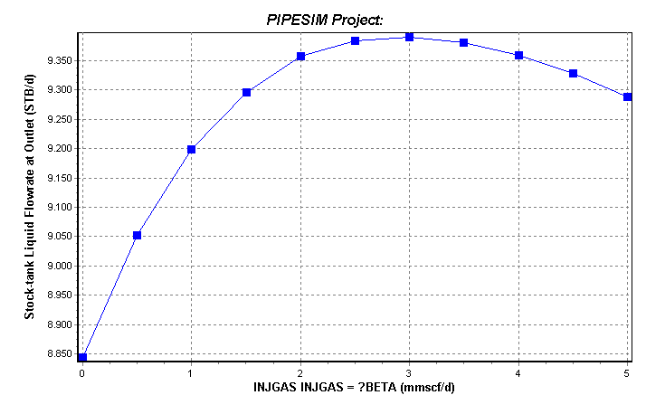
\includegraphics[height=0.7\linewidth]{figs/truth1.png}
  \caption{Curva "real" do poço de petróleo.}
  \label{fig:truth1}
\end{subfigure}
\caption{Experimento 1.}
\label{fig:setup1}
\end{figure}

Para os testes, os parametros SP (pressão estática) e Liq PI (Índice de produção de líquido) foram iniciados respecticamente em 3000 e 15.
Adicionalmente, foram impostos os seguintes limites ao solver do noMADS:
\begin{align}
MIN\_MESH\_SIZE = 5e-4\\
H\_MIN = 0.001\\
F\_TARGET = 0.00001
\end{align}
em 467 segundos (7:47 minutos) o noMADS convergiu para SP=4004.15, PI = 24.72, com a função custo em 0.896. A parada se deu pelo MIN\_MESH\_SIZE. A performance do algoritmo pode ser vista na figura \ref{fig:setup1_points}


\begin{figure}
\centering
\begin{subfigure}{0.5\textwidth}
  \centering
  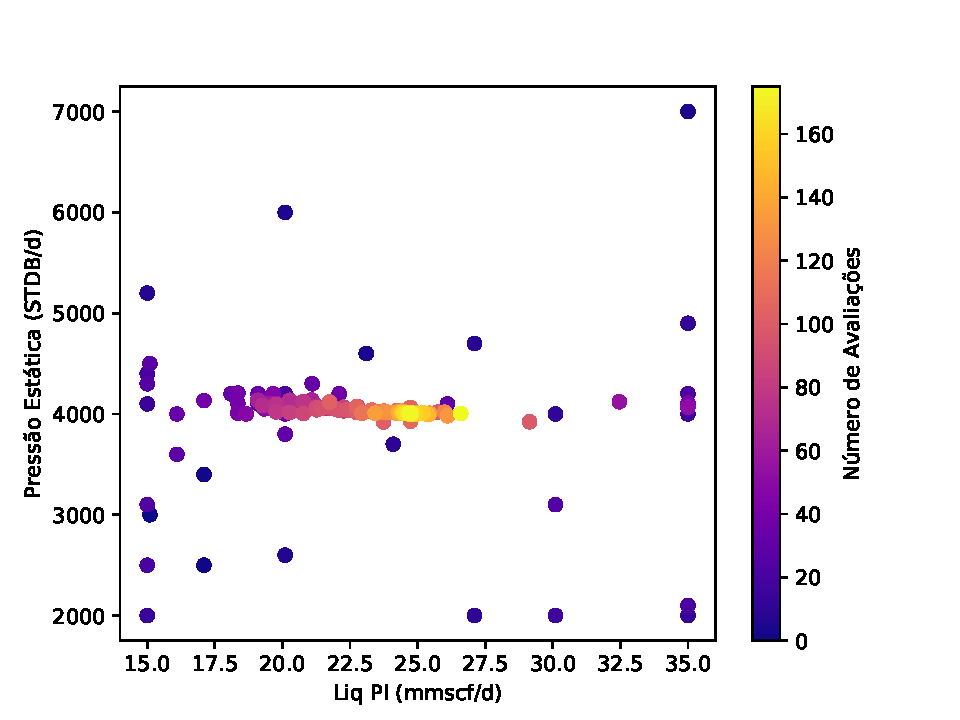
\includegraphics[width=1\linewidth]{figs/setup1_eval_points.pdf}
  \caption{Pontos escolhidos pelo noMADS.}
  \label{fig:setup1_points}
\end{subfigure}%
\begin{subfigure}{0.5\textwidth}
  \centering
  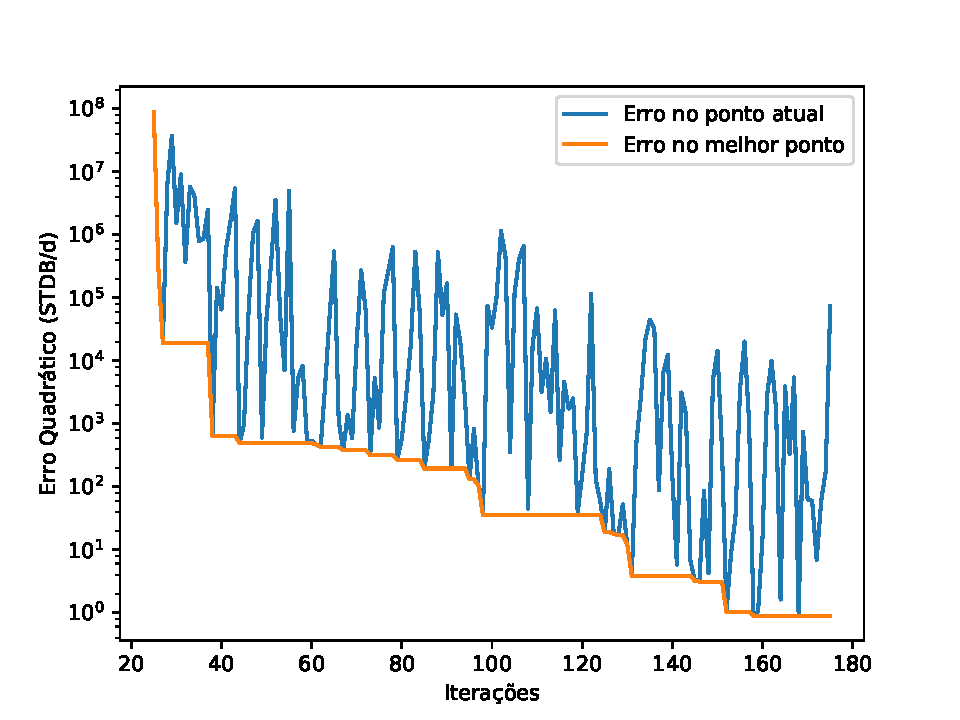
\includegraphics[width=1\linewidth]{figs/setup1_errors.pdf}
  \caption{Erro nos pontos avaliados.}
  \label{fig:setup1_error}
\end{subfigure}
\caption{Experimento 1.}
\label{fig:setup1_2}
\end{figure}


\section{Discussion}





%%%%%%%%%%%%%%%
